\documentclass{standalone}
\usepackage{tikz}
\usepackage{tabularx}
\usepackage{colortbl}
\usepackage{booktabs}

\begin{document}
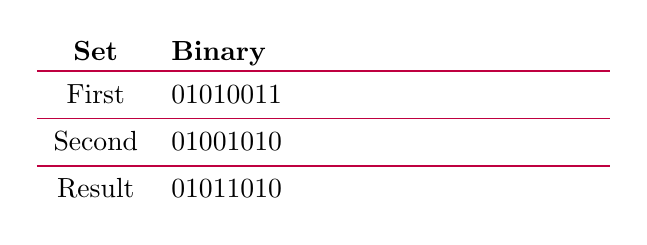
\begin{tikzpicture}

\node (tbl) {
\begin{tabularx}{.6\textwidth}{cXrcc}
\arrayrulecolor{purple}
\textbf{Set} & \textbf{Binary} \\
\toprule
First & 01010011 \\ 
\midrule
Second & 01001010 \\
\midrule
Result & 01011010  \\
\end{tabularx}
};

\end{tikzpicture}
\end{document}